\chapter{Rezultate experimentale}

Demonstratorul implementat în cadrul acestei lucrări pune față în față două arhitecturi RAG pe același set de date și același model lingvistic, cu scopul de a izola contribuția etapelor de recuperare avansată față de varianta de bază. Implementarea rulează local, pe hardware propriu, fără dependență de servicii externe sau cloud. În continuare sunt descrise mai întâi deciziile de proiectare și procesul de dezvoltare, urmate de evaluarea cantitativă a celor două sisteme și interpretarea calitativă a rezultatelor.

\subsection*{Arhitectura sistemului și deciziile de proiectare}

Ambele pipeline-uri partajează aceeași bază: datele sunt indexate offline, iar la momentul interogării se execută recuperarea și generarea. Diferența stă exclusiv în complexitatea etapei de recuperare.

Modelul lingvistic folosit este Qwen3-8B~\cite{gao2024retrievalaugmentedgenerationlargelanguage}, rulat local prin Ollama. Alegerea unui model open-source rulat local, în loc de un API extern, a fost motivată de controlul total asupra promptului de sistem și de eliminarea oricărei latențe de rețea. Qwen3 suportă un mod de gândire (``thinking mode'') care poate fi dezactivat prin directiva \texttt{/no\_think} în prompt, ceea ce a fost util pentru expansiunea interogărilor, unde nu este nevoie de raționament extins.

Modelul de embedding ales este \texttt{all-MiniLM-L6-v2}~\cite{karpukhin2020dpr}, un model compact cu 22M de parametri, antrenat pentru sarcini de regăsire semantică. Raportul calitate-viteză al acestui model îl face o alegere standard în sistemele RAG care nu au constrângeri hardware severe. Baza de date vectorială este ChromaDB, configurată cu spațiu cosinus pentru calculul similarității.

\subsection*{Setul de date}

Setul de date folosit este SQuAD (Stanford Question Answering Dataset)~\cite{rajpurkar-etal-2016-squad}, versiunea 1.1, split-ul de antrenare. SQuAD conține perechi întrebare-răspuns extrase din articole Wikipedia, unde răspunsul este un fragment de text din pasajul asociat. Această proprietate face posibilă o evaluare precisă a recuperării: se poate verifica dacă fragmentul recuperat conține răspunsul corect și provine din articolul corect, fără a depinde de judecata unui model suplimentar. La ingestie, paragrafele duplicate au fost eliminate, rezultând un corpus de paragrafe unice stocate ca fragmente individuale în ChromaDB.

\subsection*{Procesul de dezvoltare}

Implementarea a pornit cu varianta minimă funcțională: indexarea datelor SQuAD în ChromaDB și un pipeline Naive conectat la o interfață Streamlit. Interfața permite interogarea simultană a ambelor sisteme și afișarea comparativă a răspunsurilor, a fragmentelor recuperate și a scorurilor asociate.

Componentele Advanced RAG au fost adăugate treptat. Prima extensie a fost recuperarea sparse cu BM25~\cite{robertson2009bm25}. Inițial s-a folosit biblioteca \texttt{rank\_bm25}, dar aceasta a fost înlocuită cu \texttt{bm25s}, mult mai rapidă prin tokenizare batch și indexare optimizată. Indexul BM25 se calculează o singură dată și se salvează pe disc.

Configurarea cross-encoder-ului a necesitat câteva iterații: au fost testate mai multe modele, ajungând la \texttt{cross-encoder/ms-marco-MiniLM-L-6-v2}, care oferă un compromis bun între precizia re-scorării și latența de inferență. Pool-ul de candidați pentru reranking a crescut de la 20 la 40 pe parcursul dezvoltării, după ce s-a observat că un pool mai mic tăia uneori fragmentele relevante înainte ca cross-encoder-ul să le poată evalua.

Expansiunea interogărilor folosește Qwen3-1.7B, ales deliberat pentru dimensiunea redusă. Reformularea nu necesită raționament complex, dar viteza contează: apelul LLM se află pe calea critică a fiecărei interogări, iar un model de 1.7B parametri este de câteva ori mai rapid decât 8B.

Scriptul de benchmark a fost construit cu suport pentru mai multe seed-uri și checkpoint după fiecare seed, astfel încât o întrerupere să nu piardă rezultatele deja calculate. Testele de semnificație statistică (Wilcoxon și McNemar) au fost adăugate ulterior, pentru a valida că diferențele observate nu sunt artefacte ale eșantionării aleatoare.

\section{Analiză cantitativă}

\subsection{Configurarea experimentului}

Evaluarea a rulat pe câte 150 de întrebări selectate aleator din split-ul de antrenare SQuAD~\cite{rajpurkar-etal-2016-squad}, pe 4 seed-uri distincte (42, 1042, 2042, 3042), totalizând 600 de evaluări per sistem. Utilizarea mai multor seed-uri permite estimarea variabilității rezultatelor și raportarea mediei cu deviația standard.

Metricile calculate sunt:

\begin{itemize}
    \item \textbf{Context Recall@5}: fracția de întrebări pentru care cel puțin unul din cei $K{=}5$ candidați recuperați conține răspunsul corect și provine din articolul corect. Condiția privind sursa este necesară pentru a preveni potrivirile false pe fragmente scurte și frecvente (de exemplu, ``mai'' sau ``SUA'') care pot apărea în contexte complet diferite~\cite{rajpurkar-etal-2016-squad}.
    \item \textbf{Mean Reciprocal Rank (MRR)}: inversul rangului primului fragment relevant, mediat pe toate întrebările~\cite{karpukhin2020dpr}. MRR penalizează sistemele care plasează fragmentul corect pe poziții inferioare în lista de rezultate.
    \item \textbf{Answer F1}: scorul $F_1$ la nivel de token între răspunsul generat și răspunsurile de referință SQuAD, calculat ca maxim peste toate variantele de referință disponibile.
    \item \textbf{Exact Match}: proporția de răspunsuri generate care conțin textul de referință ca subșir exact, după normalizarea majusculelor și a semnelor de punctuație.
    \item \textbf{Latența medie de recuperare}: timpul de procesare a interogării în milisecunde. Pentru Advanced RAG, aceasta include apelul LLM pentru expansiunea interogării, recuperarea hibridă paralelă și re-scorarea cu cross-encoder.
\end{itemize}

Pentru testarea semnificației statistice s-au aplicat două teste pereche pe cele 600 de înregistrări combinate din toate seed-urile. Testul Wilcoxon signed-rank a fost aplicat pe metricile continue (MRR și Answer F1), iar testul McNemar pe metricile binare (Context Recall și Exact Match)~\cite{gao2024retrievalaugmentedgenerationlargelanguage}.

\subsection{Rezultate}

Rezultatele agregate pe cele 4 seed-uri sunt prezentate în Tabelul~\ref{tab:rezultate}. Advanced RAG depășește Naive RAG pe toate metricile de calitate, cu o creștere de 14,4 puncte procentuale la Context Recall (de la 83,5\% la 95,5\%), 25,7 puncte la MRR (de la 0,719 la 0,904) și 10,4 puncte la Exact Match (de la 64,2\% la 74,5\%). Answer F1 crește mai modest, cu 7,3\% relativ (de la 0,191 la 0,205).

\begin{table}[ht]
\centering
\caption{Rezultate comparative Naive RAG vs.\ Advanced RAG pe SQuAD ($N=600$ per sistem, medie $\pm$ deviație standard pe 4 seed-uri)}
\label{tab:rezultate}
\begin{tabular}{lcc}
\toprule
\textbf{Metrică} & \textbf{Naive RAG} & \textbf{Advanced RAG} \\
\midrule
Context Recall@5   & $0{,}835 \pm 0{,}006$ & $0{,}955 \pm 0{,}015$ \\
MRR                & $0{,}719 \pm 0{,}013$ & $0{,}904 \pm 0{,}023$ \\
Exact Match        & $0{,}642 \pm 0{,}027$ & $0{,}745 \pm 0{,}045$ \\
Answer F1          & $0{,}191 \pm 0{,}008$ & $0{,}205 \pm 0{,}015$ \\
Latență medie (ms) & $15{,}6  \pm 0{,}1$   & $769{,}3 \pm 20{,}8$  \\
\bottomrule
\end{tabular}
\end{table}

Figurile~\ref{fig:retrieval_metrics} și~\ref{fig:answer_quality} ilustrează grafic diferențele pentru metricile de recuperare și de calitate a răspunsurilor. Figura~\ref{fig:latency} prezintă comparativ latența medie de procesare, iar Figura~\ref{fig:radar} oferă o vedere de ansamblu a tuturor metricilor de calitate.

\begin{figure}[ht]
    \centering
    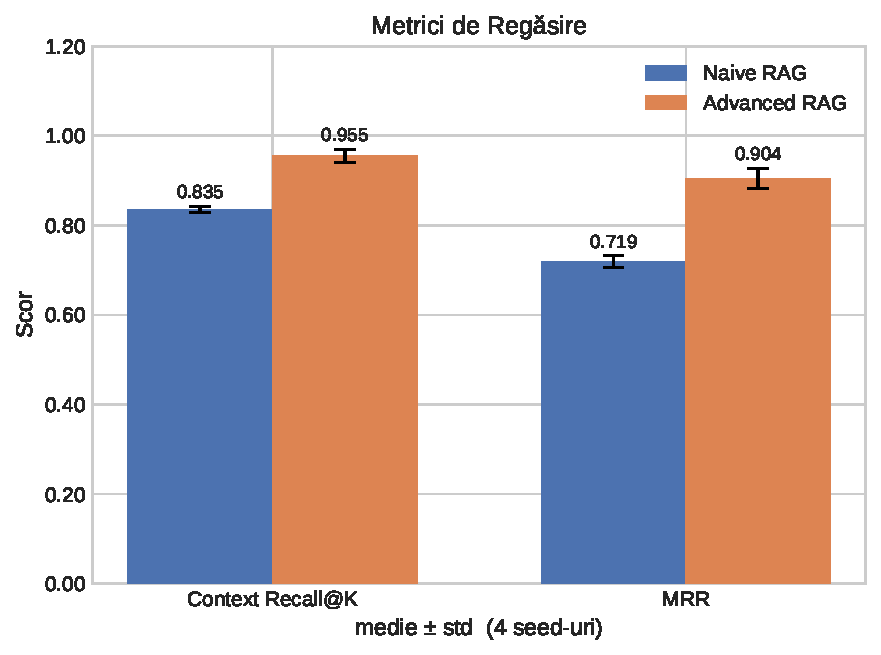
\includegraphics[width=0.80\linewidth]{Imagini/retrieval_metrics.pdf}
    \caption{Metrici de recuperare: Context Recall@5 și MRR pentru Naive RAG și Advanced RAG. Barele de eroare reprezintă deviația standard calculată pe cele 4 seed-uri.}
    \label{fig:retrieval_metrics}
\end{figure}

\begin{figure}[ht]
    \centering
    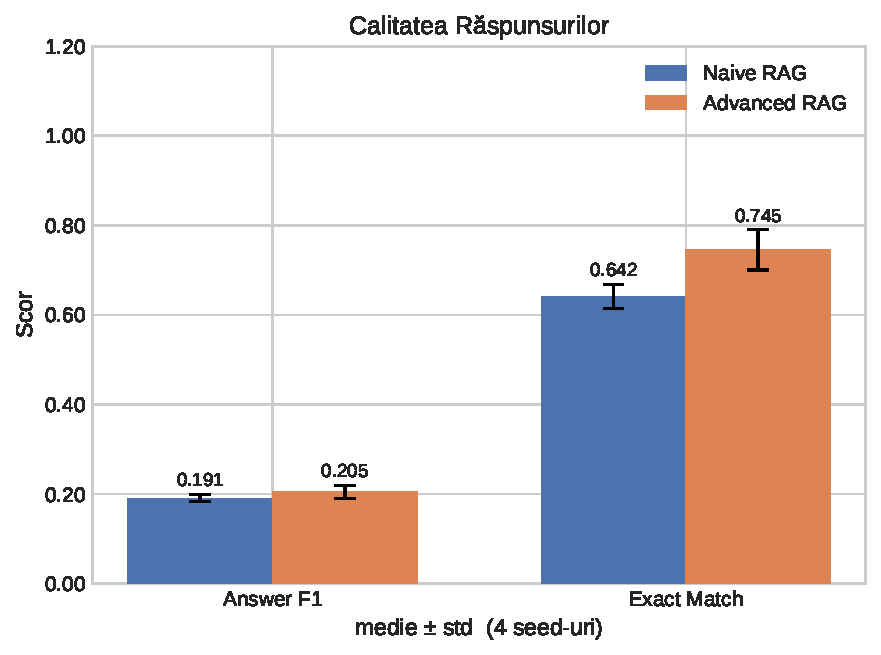
\includegraphics[width=0.80\linewidth]{Imagini/answer_quality.pdf}
    \caption{Calitatea răspunsurilor: Answer F1 și Exact Match pentru Naive RAG și Advanced RAG.}
    \label{fig:answer_quality}
\end{figure}

\begin{figure}[ht]
    \centering
    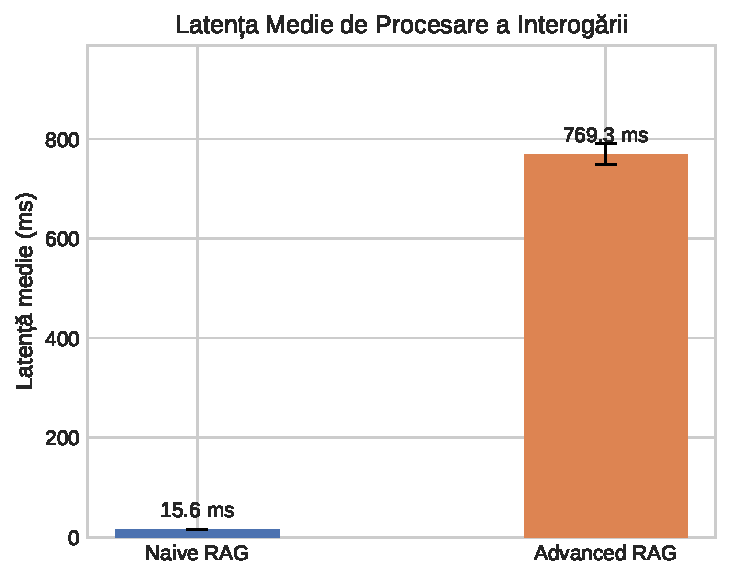
\includegraphics[width=0.65\linewidth]{Imagini/latency.pdf}
    \caption{Latența medie de procesare a interogării în milisecunde. Latența Advanced RAG include apelul LLM pentru expansiunea interogării, recuperarea hibridă paralelă și re-scorarea cu cross-encoder.}
    \label{fig:latency}
\end{figure}

\begin{figure}[ht]
    \centering
    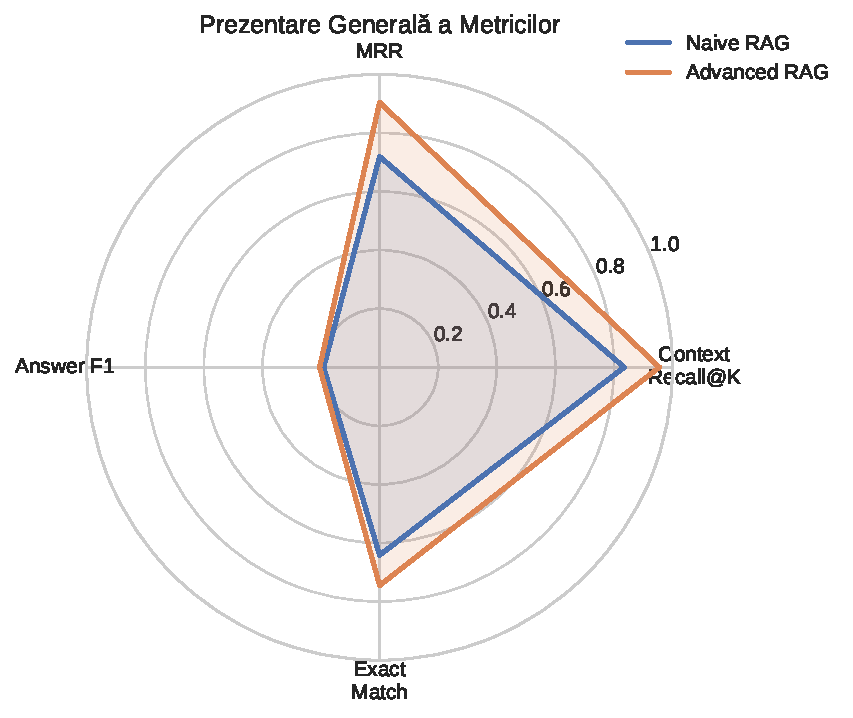
\includegraphics[width=0.72\linewidth]{Imagini/overview_radar.pdf}
    \caption{Vedere de ansamblu comparativă a metricilor de calitate (Context Recall@5, MRR, Answer F1, Exact Match). Latența nu este inclusă deoarece se află pe o scară diferită (milisecunde față de 0--1).}
    \label{fig:radar}
\end{figure}

\subsection{Semnificație statistică}

Toate diferențele observate sunt semnificative statistic la $p < 0{,}05$, cu marje considerabile față de prag (Tabelul~\ref{tab:significance}).

\begin{table}[ht]
\centering
\caption{Teste de semnificație statistică (Advanced RAG vs.\ Naive RAG, $N=600$ perechi)}
\label{tab:significance}
\begin{tabular}{lccl}
\toprule
\textbf{Metrică} & \textbf{Test} & \textbf{Valoarea $p$} & \textbf{Observații} \\
\midrule
MRR            & Wilcoxon & $6{,}5 \times 10^{-27}$ & --- \\
Answer F1      & Wilcoxon & $1{,}8 \times 10^{-3}$  & --- \\
Context Recall & McNemar  & $7{,}7 \times 10^{-20}$ & Adv.\ mai bun: 74; Naive mai bun: 2 \\
Exact Match    & McNemar  & $4{,}3 \times 10^{-10}$ & Adv.\ mai bun: 82; Naive mai bun: 20 \\
\bottomrule
\end{tabular}
\end{table}

Valoarea $p$ extrem de mică pentru MRR ($6{,}5 \times 10^{-27}$) indică o diferență sistematică, nu un artefact al eșantionării. Testul McNemar pentru Context Recall arată că există 74 de întrebări unde Advanced RAG recuperează fragmentul corect, iar Naive RAG nu reușește, față de doar 2 în situația inversă. Raportul de 37:1 în favoarea sistemului avansat confirmă că îmbunătățirile în recuperare nu provin din cazuri marginale, ci reprezintă un avantaj consistent.

\section{Analiză calitativă}

\subsection{Compromisul dintre calitate și latență}

Cel mai vizibil cost al arhitecturii avansate este latența de recuperare: 769 ms față de 16 ms pentru varianta de bază, o creștere de aproximativ 50 de ori. Această diferență are câteva surse distincte. Expansiunea interogărilor implică un apel LLM (Qwen3-1.7B), care durează câteva sute de milisecunde chiar și pentru un model de 1.7B parametri. Recuperarea densă și BM25 rulează în paralel pe toate cele trei formulări (originală plus două alternative), ceea ce limitează parțial impactul, dar cross-encoder-ul introduce o latentă suplimentară pentru re-scorarea celor 40 de candidați.

În contextul aplicațiilor RAG reale, o latență de recuperare de ~770 ms rămâne acceptabilă, deoarece generarea unui răspuns cu un model de 8B parametri durează oricum mai multe secunde. Totuși, în scenarii unde se doresc timpi de răspuns sub o secundă, overhead-ul expansiunii interogărilor devine o constrângere reală și ar putea fi eliminat printr-o versiune fără expansiune, care combină recuperarea hibridă fără reformulare~\cite{gao2024retrievalaugmentedgenerationlargelanguage}.

\subsection{Unde ajută recuperarea hibridă}

Diferența cea mai pronunțată dintre cele două sisteme apare la metricile de recuperare, nu la cele de generare. Creșterea cu 14,4 puncte la Context Recall înseamnă că, în 12 din 100 de cazuri unde Naive RAG eșuează, Advanced RAG găsește totuși fragmentul corect. MRR crescut de la 0,719 la 0,904 arată că, pe lângă faptul că găsește mai des fragmentul corect, îl și plasează pe poziții mai înalte.

Recuperarea hibridă (densă + BM25) are un avantaj clar pe interogările cu termeni specifici: date, numere, denumiri proprii, acronime. Modelul de embedding codifică înțeles semantic, dar poate dilua termeni rari într-un spațiu vectorial continuu unde similaritatea cosinus favorizează documente tematic apropiate, nu neapărat lexical identice. BM25~\cite{robertson2009bm25} nu are această problemă: un termen care apare exact o dată în corpus va fi regăsit cu precizie dacă apare și în interogare. Expansiunea interogărilor contribuie la recall prin acoperirea variantelor de formulare, reducând dependența de formularea exactă a întrebării~\cite{gao2024retrievalaugmentedgenerationlargelanguage}.

\subsection{Decalajul dintre recuperare și generare}

Îmbunătățirile la recuperare nu se traduc proporțional în îmbunătățiri la generare. Context Recall crește cu ~14 puncte procentuale, dar Answer F1 crește cu ~7\% relativ, iar Exact Match cu ~10 puncte procentuale.

Explicația principală este că SQuAD a fost conceput ca benchmark pentru citire extractivă, unde modelul ar trebui să extragă textual un fragment din pasaj. Modelele generative moderne tind să parafrazeze răspunsul mai degrabă decât să îl reproducă cuvânt cu cuvânt, ceea ce scade Answer F1 față de valoarea maximă posibilă, chiar dacă răspunsul este corect semantic. O a doua explicație este că Naive RAG recuperează corect fragmentul în 83,5\% din cazuri, ceea ce înseamnă că modelul generativ primea oricum contextul corect pentru cea mai mare parte a întrebărilor. Câștigul din Advanced RAG vine tocmai din cazurile dificile, adică interogările cu termeni rari sau cu răspunsuri scurte greu de localizat prin similaritate semantică pură, unde generarea oricum eșuează mai des.

\subsection{Constrângerea de groundare și refuzurile}

Ambele pipeline-uri folosesc un prompt de sistem care constrânge modelul să răspundă exclusiv din contextul furnizat și să refuze explicit dacă informația lipsește. Exact promtul de refuz este: \textit{``The provided context does not contain enough information to answer this question.''} Această decizie de proiectare este direct motivată de principiul fidelității contextuale descris în~\cite{asai2023self}: un sistem care preferă să refuze decât să inventeze este mai fiabil decât unul care generează răspunsuri plauzibile dar incorecte.

Refuzurile nu pot fi evaluate cu Answer F1 sau Exact Match, deoarece nu conțin conținut factual comparabil cu referința. Advanced RAG generează mai puține refuzuri decât Naive RAG, pentru că recuperează mai frecvent fragmentul corect și îl plasează pe primele poziții, astfel că modelul primește mai rar un context din care nu poate răspunde.

\subsection{Observații calitative din interfața Streamlit}

Interfața Streamlit permite observarea directă a diferențelor de comportament fără a parcurge metricile agregate.

Pe întrebări cu termeni numerici sau coduri specifice (``Câte specii...'', ``În ce an...'', ``Care este codul...''), Naive RAG returnează adesea fragmente tematic relevante care nu conțin numărul exact. Advanced RAG găsește fragmentul corect prin BM25, care tratează numerele ca termeni distincți și nu le diluează în spațiu vectorial.

Când răspunsul nu există în corpus, ambele sisteme refuză explicit. Diferența este că Advanced RAG produce mai rar răspunsuri parțiale construite din context adiacent irelevant, deoarece cross-encoder-ul elimină candidații slab relevanți înainte de generare.

Pe întrebări tematice generale (``Despre ce este...'', ``Care este rolul...''), ambele sisteme produc rezultate similare. Recuperarea densă funcționează bine pe similitudine semantică, iar avantajul hibridizării este mai puțin pronunțat în aceste cazuri.

Aceste observații sunt consistente cu rezultatele cantitative: câștigurile Advanced RAG sunt mai mari pe cazurile dificile (termeni rari, răspunsuri numerice) și mai mici pe interogările tematice generale, unde recuperarea densă funcționează deja bine~\cite{gao2024retrievalaugmentedgenerationlargelanguage,robertson2009bm25}.
